%!TEX root=report.tex

\subsection{time series analysis - ARIMA}

To get an indication if its possible to use time series analysis on the GRACE data, a single position (63.5 N 49.5 W, west coast of Greenland) have been selected.

To analyze the data using an ARIMA model an equidistant dataset is required. For example it would otherwise not possible to solve the Yule-Walker equations \cite[s.~122]{time-series-analysis}. In the original GRACE dataset some values are missing, thus they should be interpolated. Also in order to get an indication of the model performance, the last 36 observations (a year) have been separated for cross validation testing.

\begin{figure}[H]
\centering
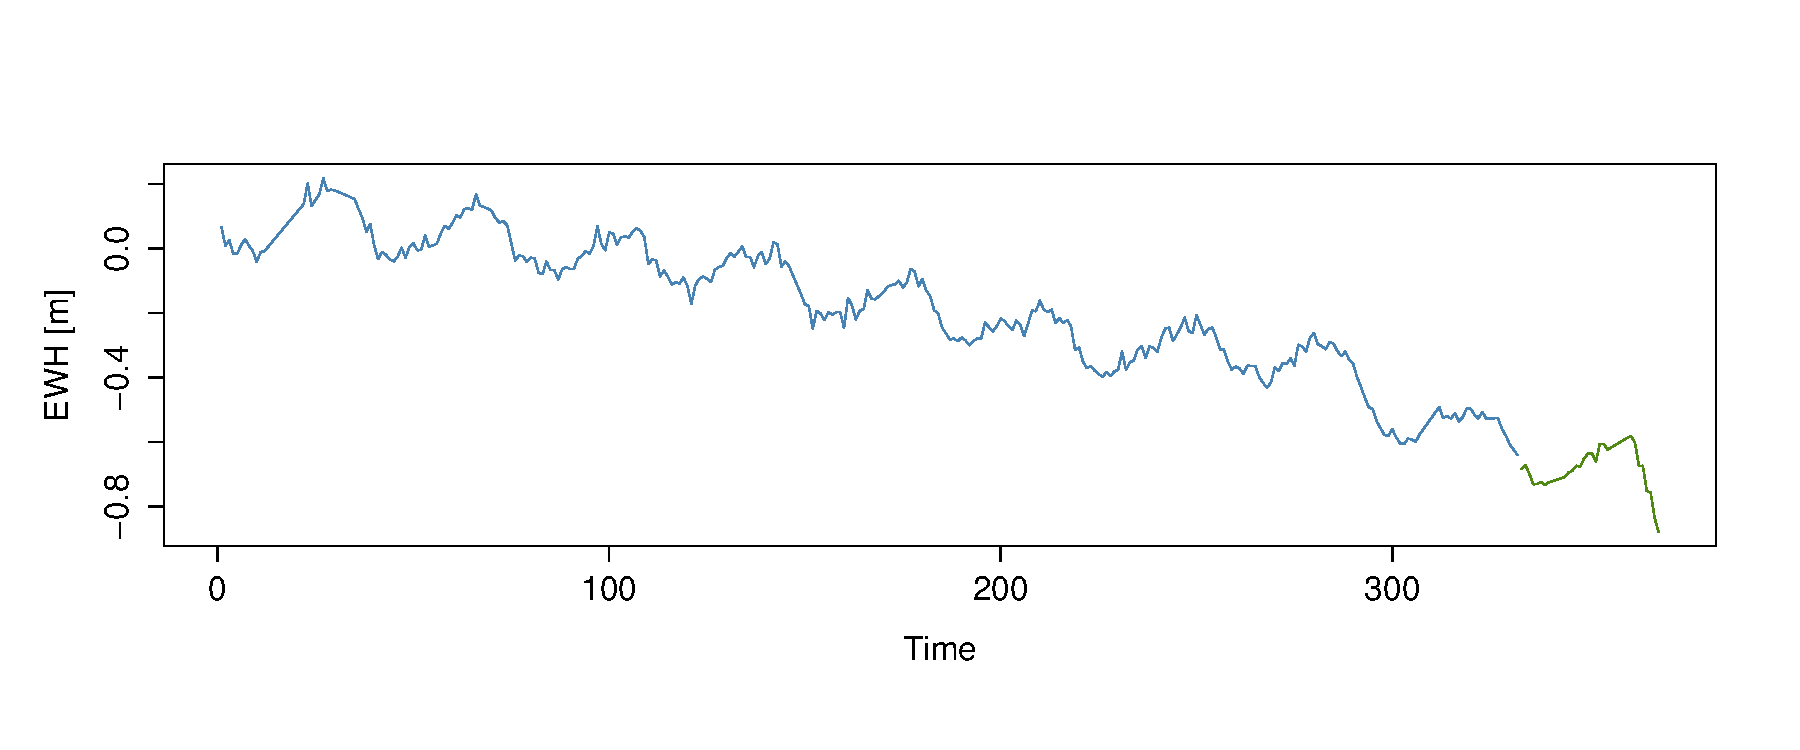
\includegraphics[height=5cm]{figures/ts-initial-split}
\caption{GRACE data at 63.5 N 49.5 W, where missing values are interpolated. Blue is the training data and green is the  test data.}
\label{fig:ts-initial-split}
\end{figure}

The time series in Figure \ref{fig:ts-initial-split} is clearly not stationary, thus it is necessary to consider the time series difference.
\begin{figure}[H]
\centering
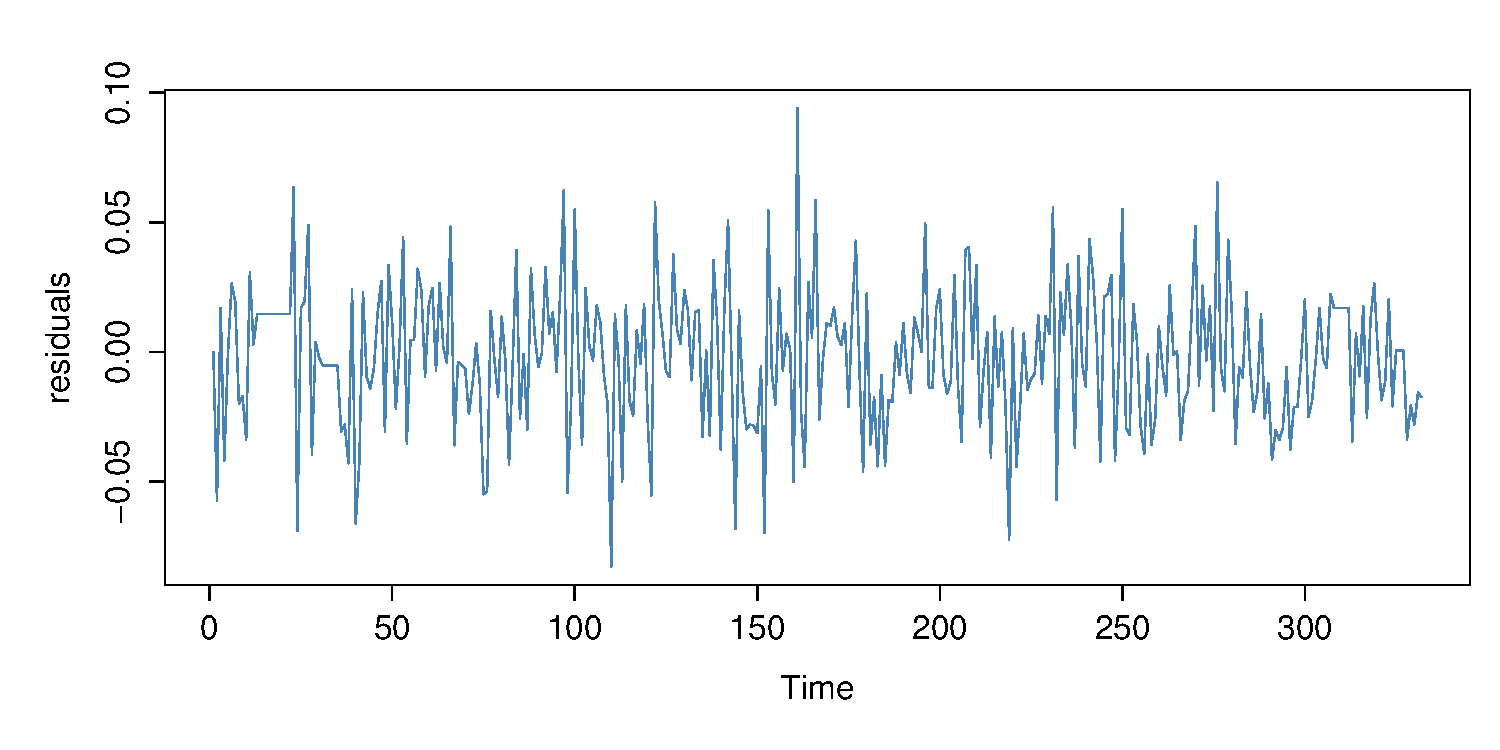
\includegraphics[height=5cm]{figures/ts-residual-i1s0}
\caption{The ARIMA$(0,1,0) \times (0,0,0)_{36}$ residuals.}
\label{fig:ts-residual-i1s0}
\end{figure}
On Figure \ref{fig:ts-residual-i1s0} there some seasonal periods where the mean and variance isn't the same as the remaining period, thus it is not completely stationary. Taking also the seasonal difference (assuming the season is 36 observations, a year) gives however a very stationary output.

\begin{figure}[H]
\centering
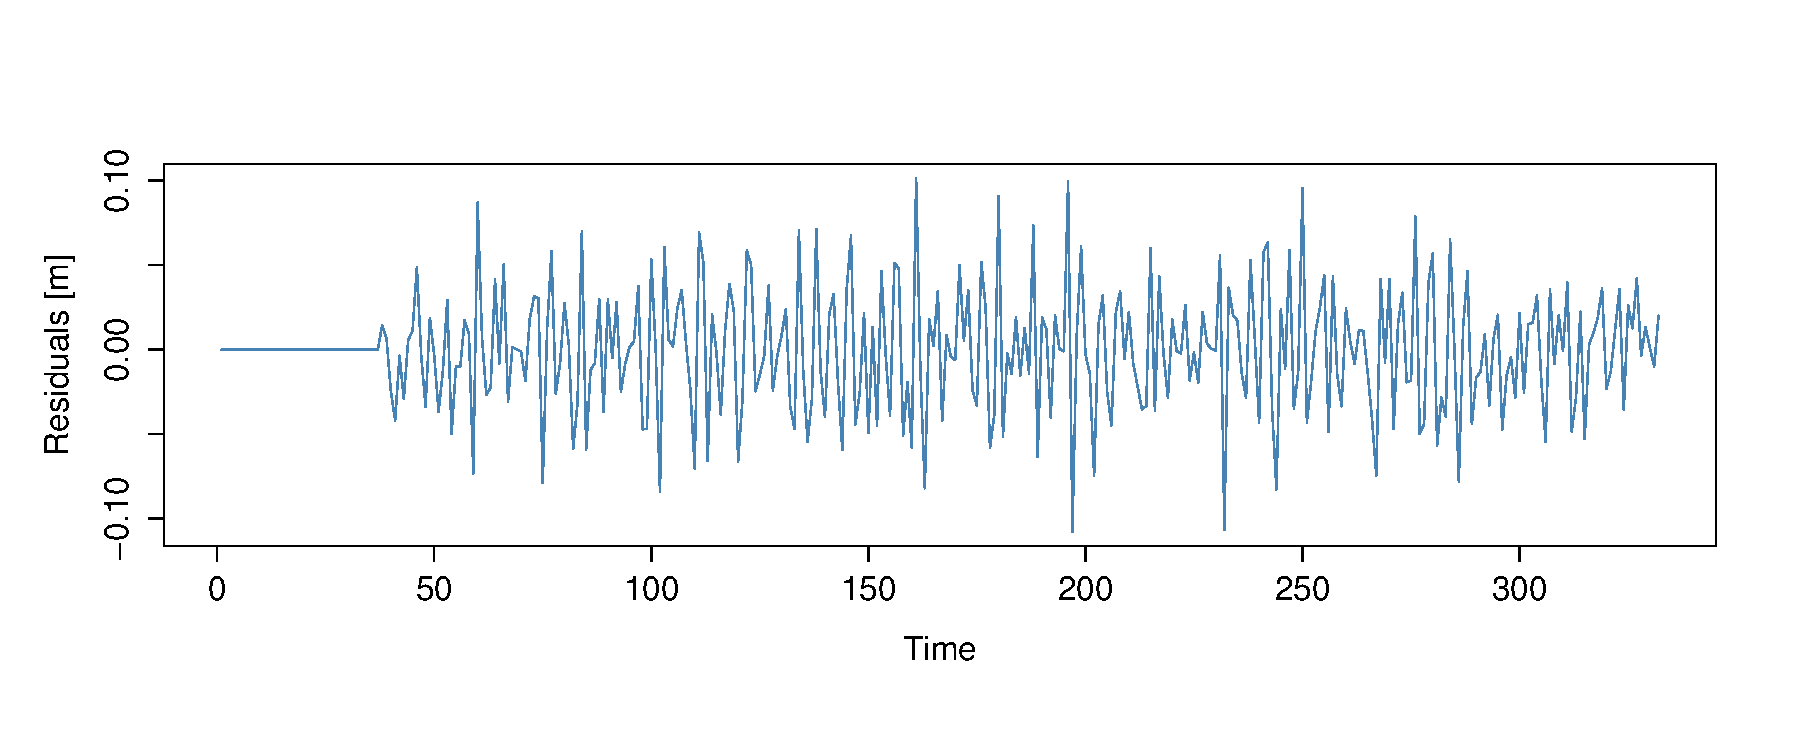
\includegraphics[height=5cm]{figures/ts-residual-i1s1}
\caption{The ARIMA$(0,1,0) \times (0,1,0)_{36}$ residuals.}
\label{fig:ts-residual-i1s1}
\end{figure}
On Figure \ref{fig:ts-residual-i1s1} its seen that the first 37 observations acts strange, this is because there aren't enough past observations to estimate the EWH correctly, thus they should be excluded from further analysis.

To determine the AR and MA terms in the ARIMA mode, the ACF and PACF should be estimated using the residuals from Figure \ref{fig:ts-residual-i1s1}.
\begin{figure}[H]
	\centering
	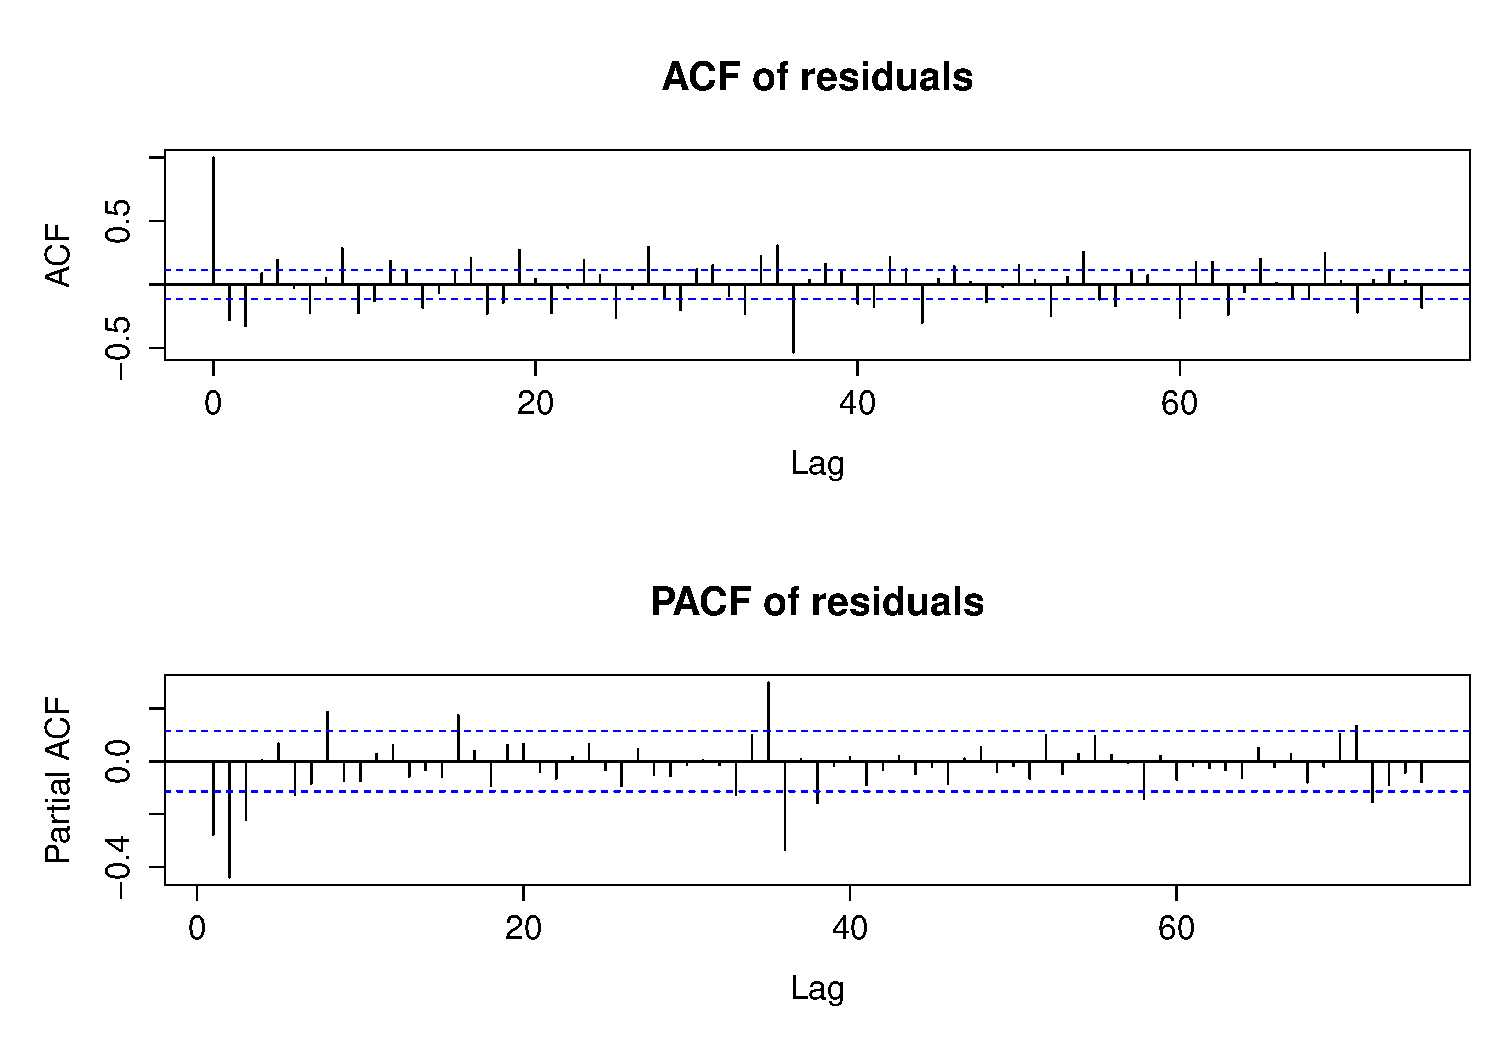
\includegraphics[width=\textwidth]{figures/ts-acf-ar0s0}
	\caption{ACF and PACF for ARIMA$(0,1,0) \times (0,1,0)_{36}$ residuals}
	\label{fig:ts-acf-ar0s0}
\end{figure}

Using the PACF in Figure \ref{fig:ts-acf-ar0s0} and the rules for the AR term \cite[Table~6.1]{time-series-analysis} \texttt{AR(2)}, seams like a good guess for the non-seasonal AR term.
\begin{figure}[H]
	\centering
	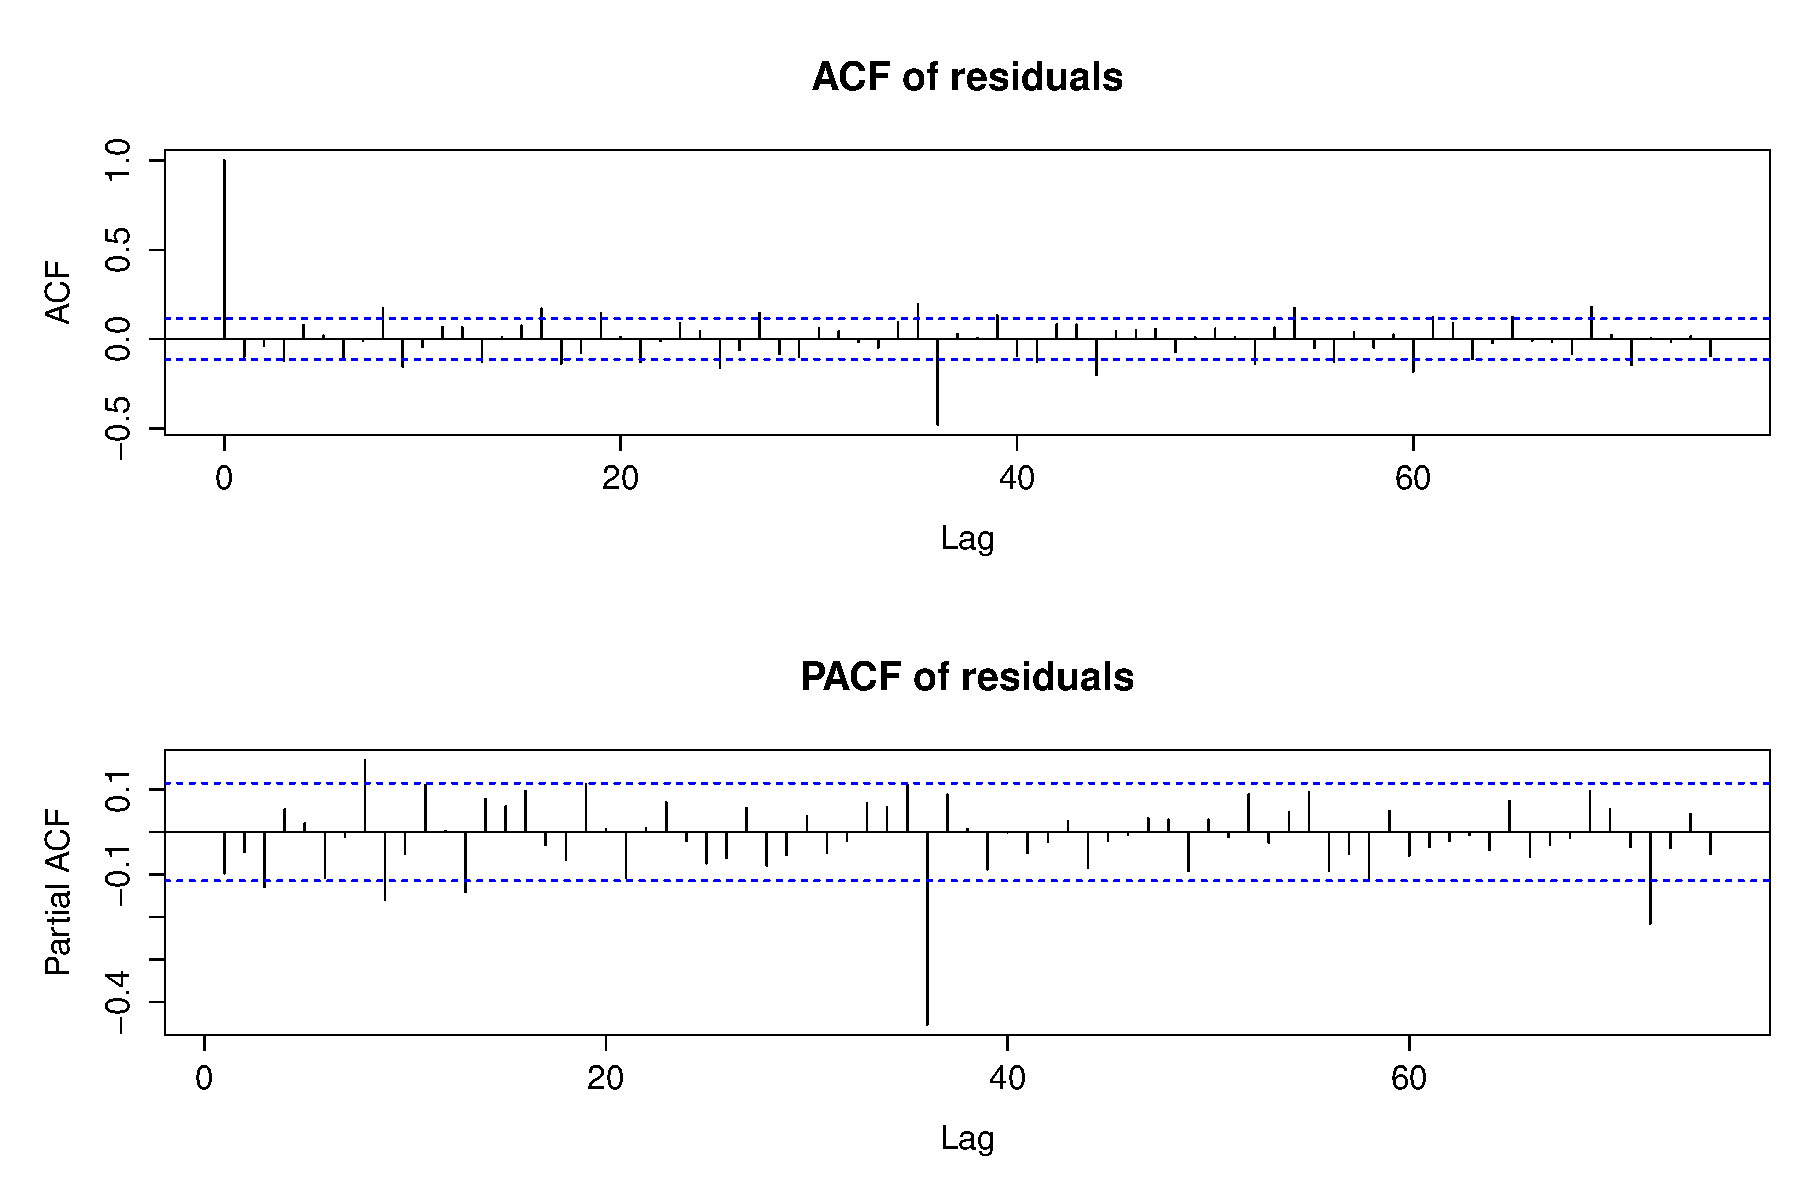
\includegraphics[width=\textwidth]{figures/ts-acf-ar2s0}
	\caption{ACF and PACF for ARIMA$(2,1,0) \times (0,1,0)_{36}$ residuals}
	\label{fig:ts-acf-ar2s0}
\end{figure}

This clearly fitted the non-seasonal trend. From Figure \ref{fig:ts-acf-ar0s0} it might have looked like there was a \texttt{AR(3)} or \texttt{MA(2)} term, but the \texttt{AR(2)} is the simplest of those and fit the trend just fine. The seasonal part is now extremely apparent in Figure \ref{fig:ts-acf-ar2s0}, where it looks like either an \texttt{SAR(2)}.
\begin{figure}[H]
	\centering
	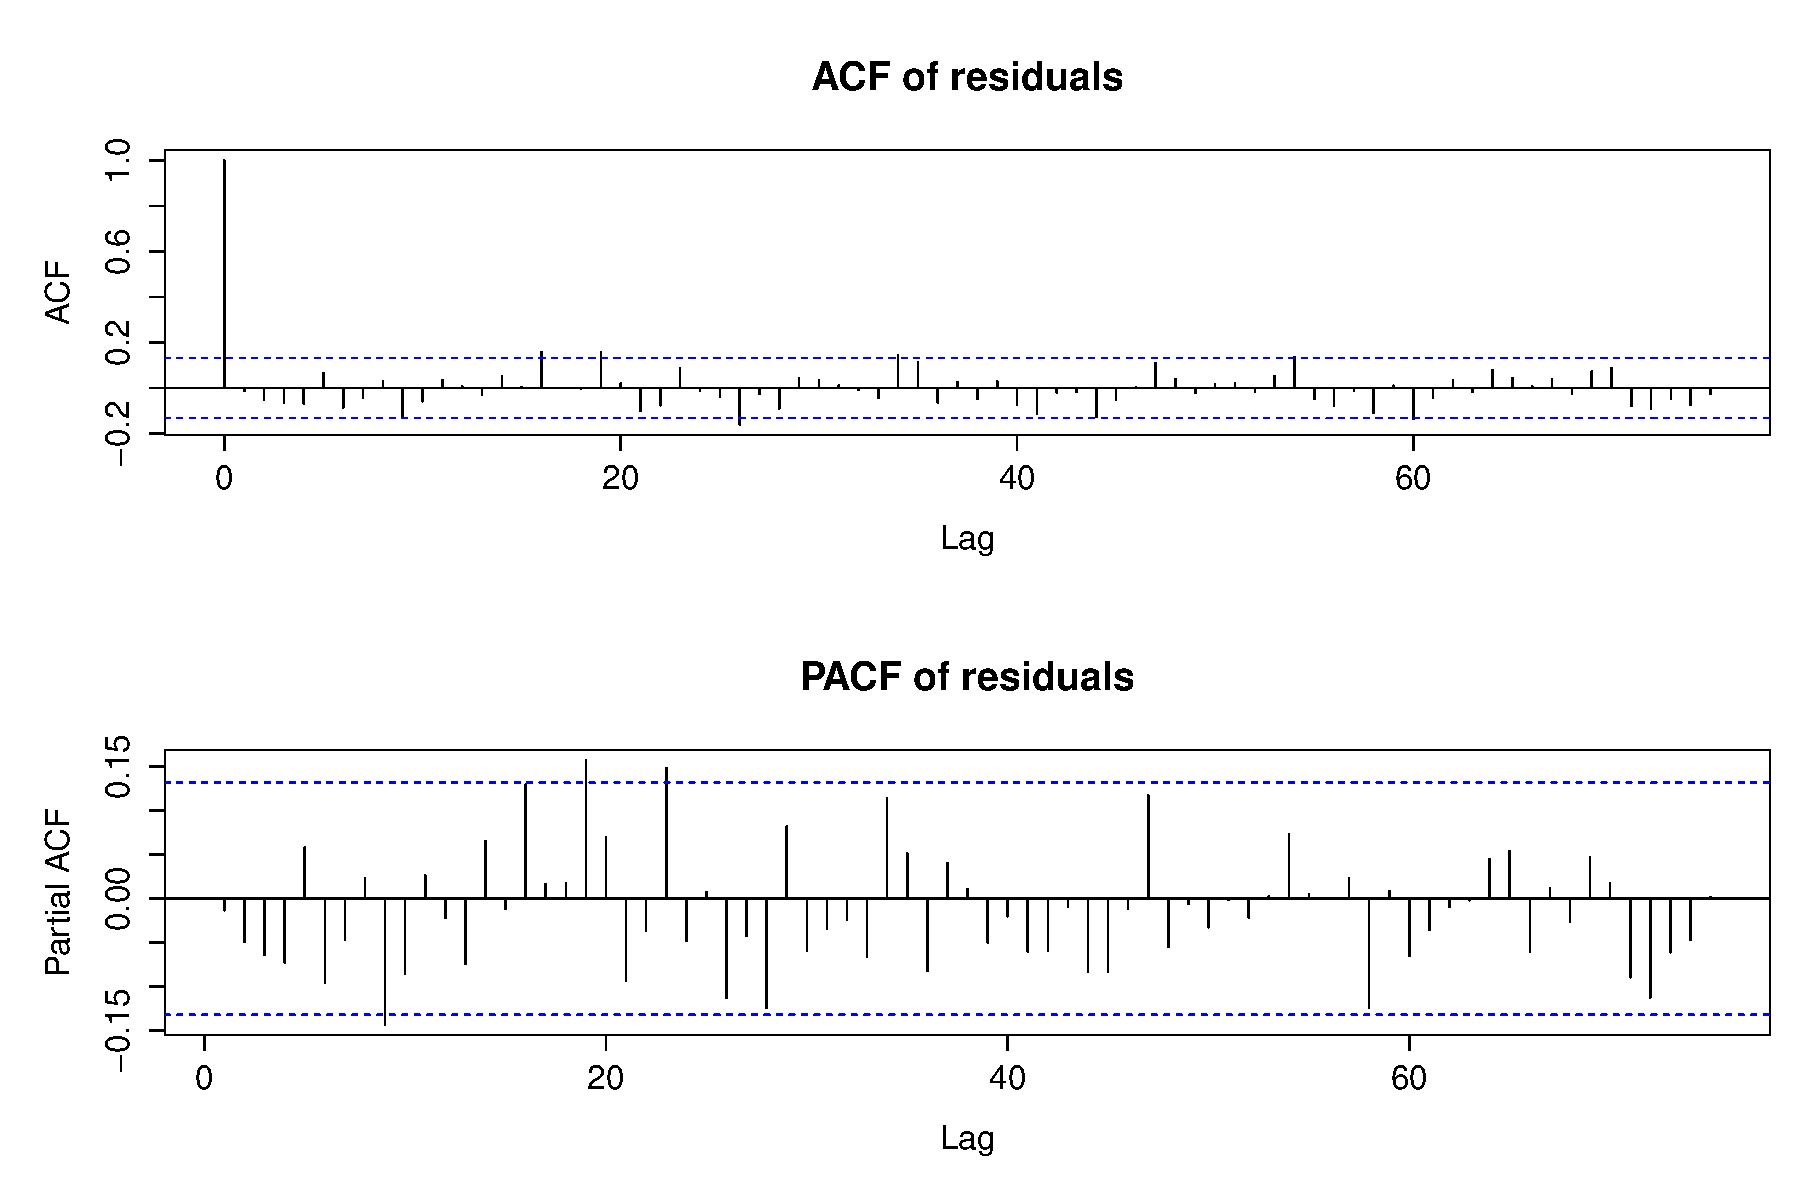
\includegraphics[width=\textwidth]{figures/ts-acf-ar2s2}
	\caption{ACF and PACF for ARIMA$(2,1,0) \times (2,1,0)_{36}$ residuals}
	\label{fig:ts-acf-ar2s2}
\end{figure}

From just looking at the estimated ACF and PACF in Figure \ref{fig:ts-acf-ar2s2}, ARIMA$(2,1,0) \times (2,1,0)_{36}$ seams like a good choice. To finally validate the model, a good start is to look at the residuals.
\begin{figure}[H]
	\centering
	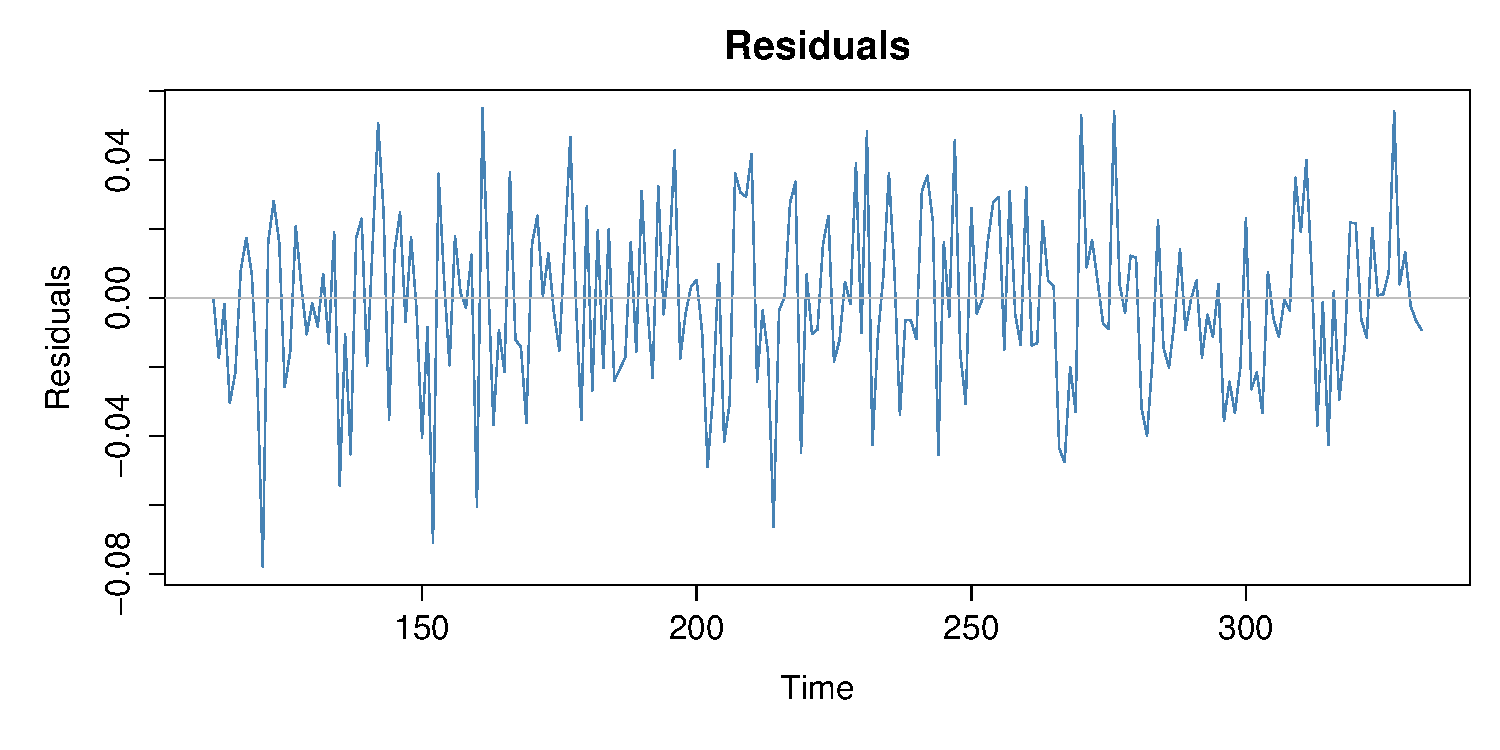
\includegraphics[height=5cm]{figures/ts-final-residual}
	\caption{ARIMA$(2,1,0) \times (2,1,0)_{36}$ residuals. The first 111 residuals have been skipped since they can't be estimated correctly.}
	\label{fig:ts-final-residual}
\end{figure}

Figure \ref{fig:ts-final-residual} looks stationary, there are no outliers nor seasonal trends. To validate the model further the Ljung-Box test can be used. This however requires the residuals to be normally distributed, a QQ-plot (Figure \ref{fig:ts-final-qq}) shows that this is the case:
\begin{figure}[H]
	\centering
	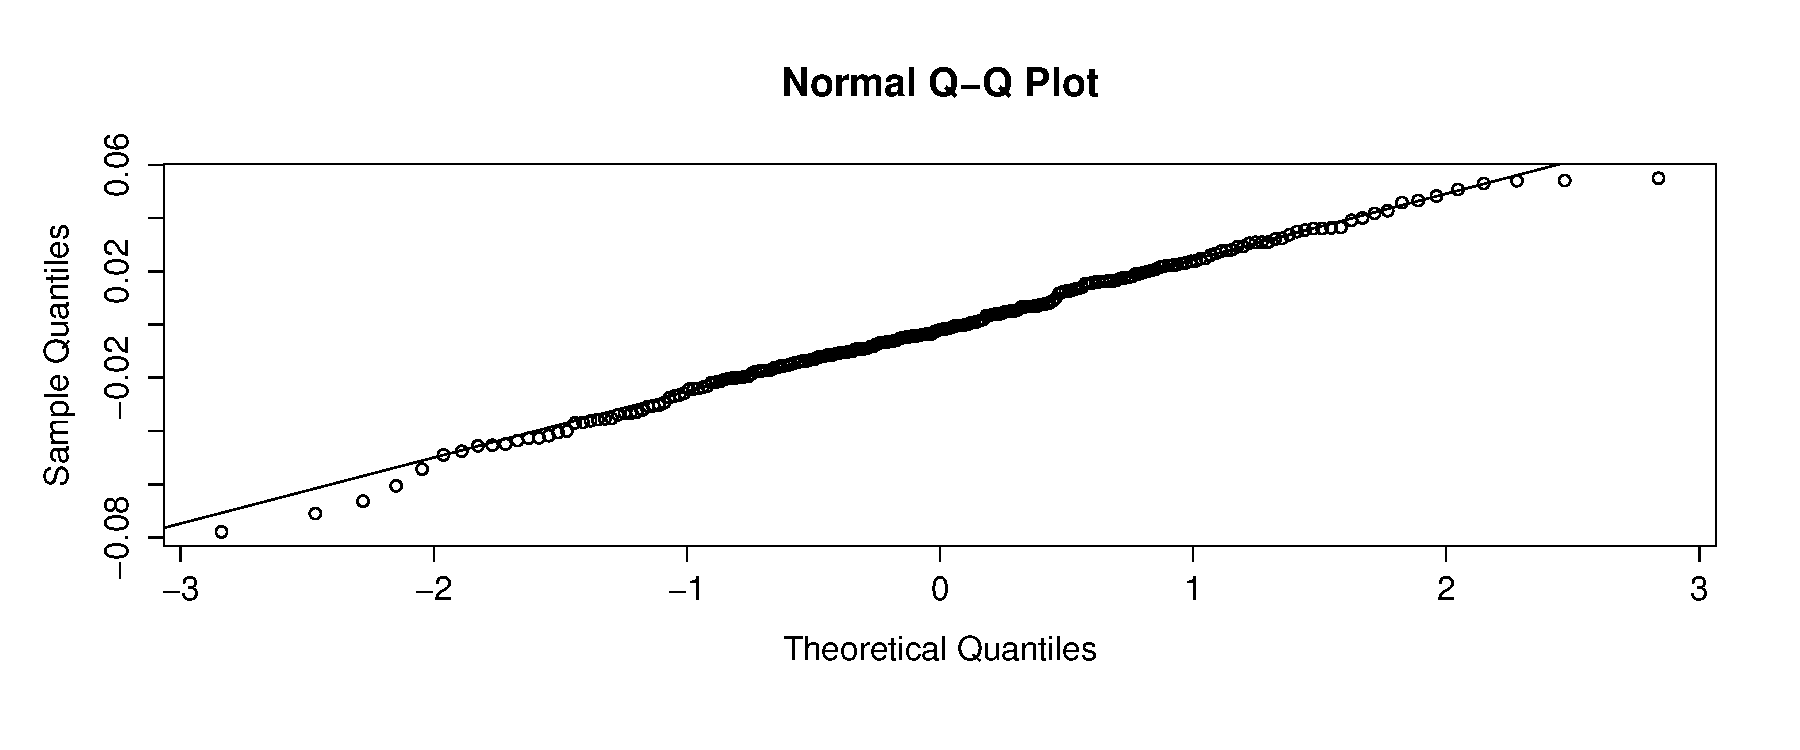
\includegraphics[height=5cm]{figures/ts-final-qq}
	\caption{QQ-plot for the ARIMA$(2,1,0) \times (2,1,0)_{36}$ residuals.}
	\label{fig:ts-final-qq}
\end{figure}

\begin{figure}[H]
	\centering
	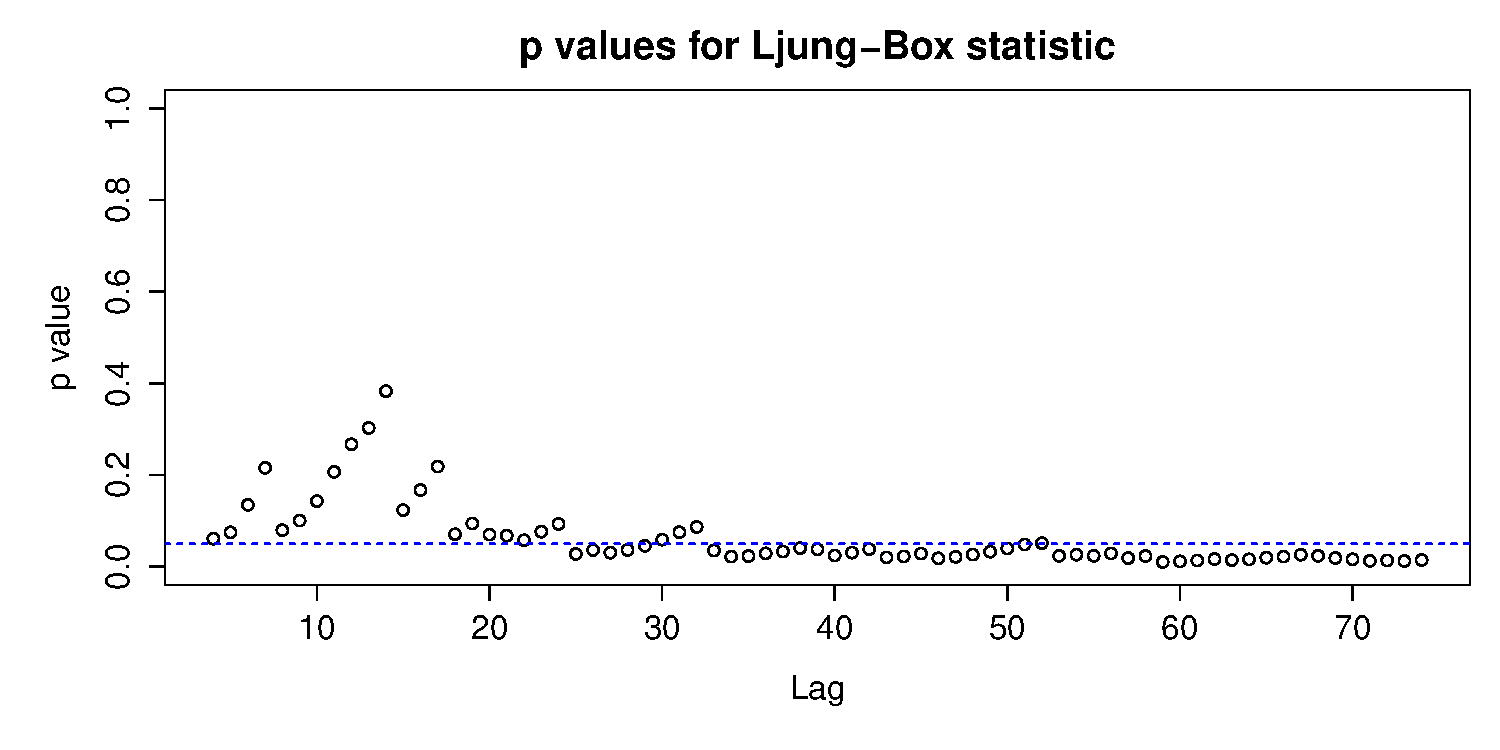
\includegraphics[height=5cm]{figures/ts-final-ljungbox}
	\caption{Ljung-Box test for the ARIMA$(2,1,0) \times (2,1,0)_{36}$ residuals.}
	\label{fig:ts-final-ljungbox}
\end{figure}

From the Ljung-Box test (Figure \ref{fig:ts-final-ljungbox}) the p-value for the first many lags looks good, however after 25 it can be with 95\% confidence statically significant concluded that the residuals are correlated. In terms of pure time series analysis is makes the model quite useless, however it is still valuable to do the cross validation.

\begin{figure}[H]
\centering
\centerline{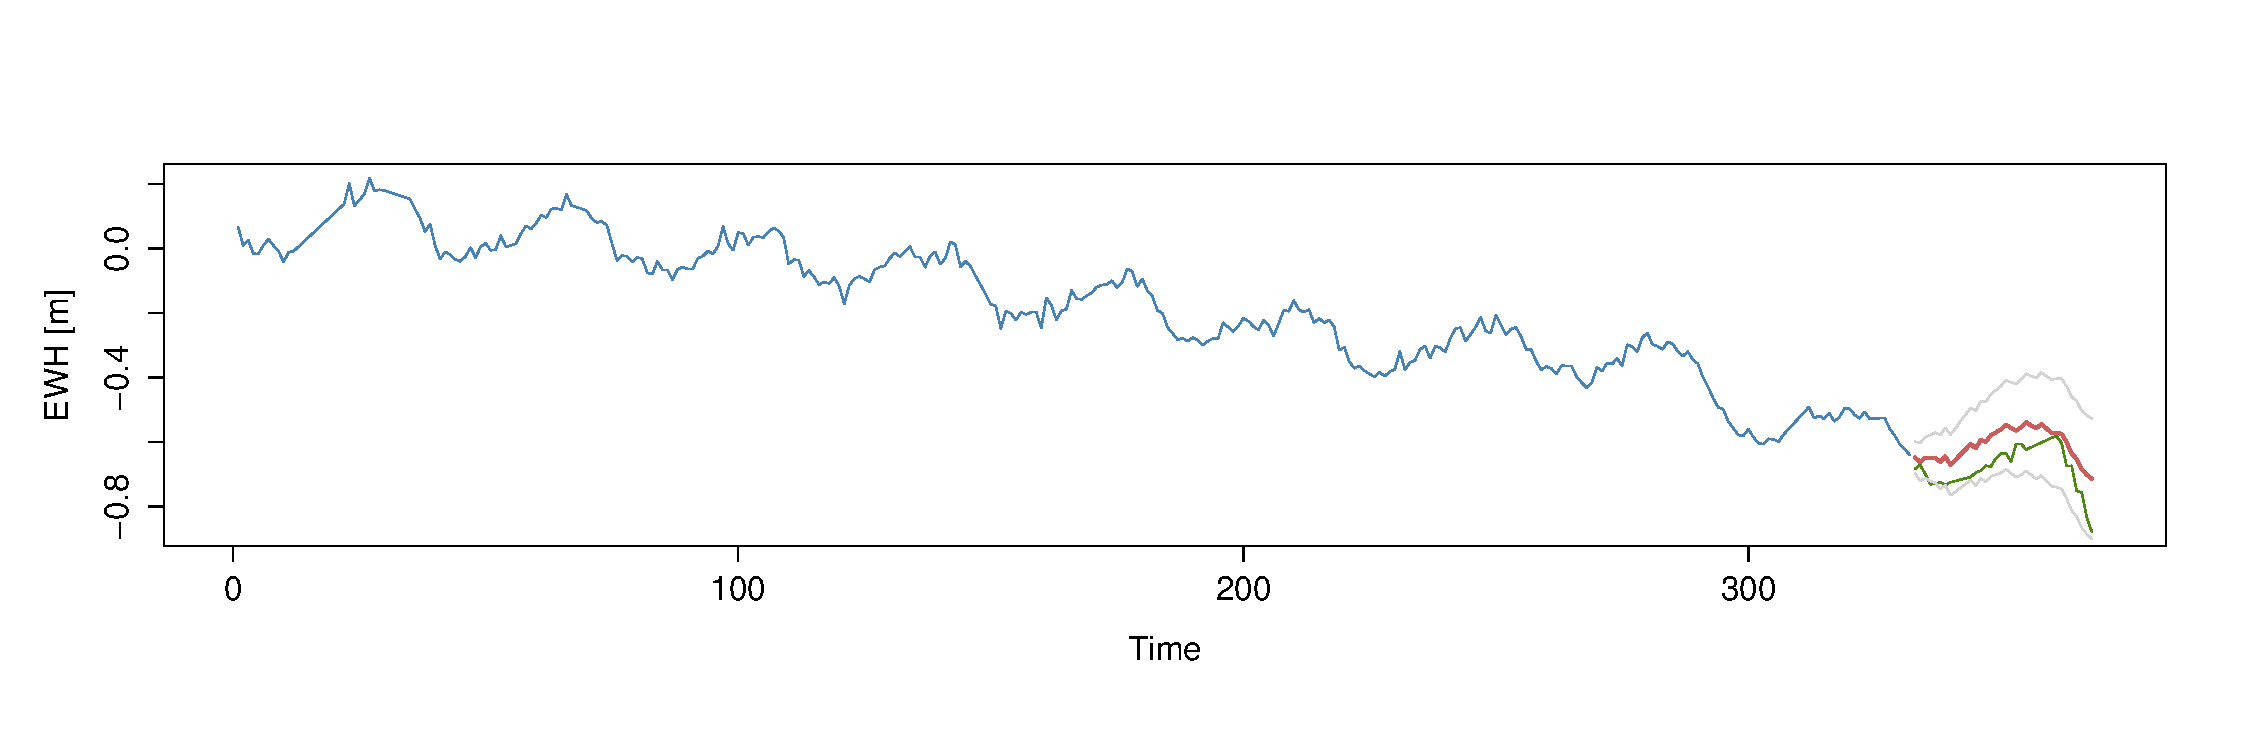
\includegraphics[height=5cm]{figures/ts-final-forecast}}
\caption{Forecast on Cross Validation. Blue is the training data, green is the test data. Red is then the predicted test values with its 95\% confidence interval marked with gray lines.}
\label{fig:ts-final-forecast}
\end{figure}

From Figure \ref{fig:ts-final-forecast} it quite clear that the test data is consistently bellow the expectation line (red). While it is still inside the 95\% confidence interval, this high correlation in the error between lags indicates that the model isn't particular useful. 
